\documentclass[a4paper,11pt]{exam}
\printanswers % pour imprimer les réponses (corrigé)
%\noprintanswers % Pour ne pas imprimer les réponses (énoncé)
\addpoints % Pour compter les points
% \noaddpoints % pour ne pas compter les points
%\qformat{\textbf{\thequestion ) } }
\qformat{\textbf{\thequestion )}} % Pour définir le style des questions (facultatif)
\usepackage{color} % définit une nouvelle couleur
\shadedsolutions % définit le style des réponses
% \framedsolutions % définit le style des réponses
\definecolor{SolutionColor}{rgb}{0.8,0.9,1} % bleu ciel
\renewcommand{\solutiontitle}{\noindent\textbf{Solution:}\par\noindent} % Définit le titre des solutions




\makeatletter

\def\maketitle{{\centering%
	\par{\huge\textbf{\@title}}%
	\par{\@date}%
	\par}}

\makeatother

\lhead{NOM Pr\'enom :}
\rhead{\textbf{Les r\'eponses doivent \^etre justifi\'ees}}
\cfoot{\thepage / \pageref{LastPage}}


%\usepackage{../../pas-math}
%\usepackage{../../moncours}


%\usepackage{pas-cours}
%-------------------------------------------------------------------------------
%          -Packages nécessaires pour écrire en Français et en UTF8-
%-------------------------------------------------------------------------------
\usepackage[utf8]{inputenc}
\usepackage[frenchb]{babel}
\usepackage[T1]{fontenc}
\usepackage{lmodern}
\usepackage{textcomp}



%-------------------------------------------------------------------------------

%-------------------------------------------------------------------------------
%                          -Outils de mise en forme-
%-------------------------------------------------------------------------------
\usepackage{hyperref}
\hypersetup{pdfstartview=XYZ}
%\usepackage{enumerate}
\usepackage{graphicx}
\usepackage{multicol}
\usepackage{tabularx}
\usepackage{multirow}


\usepackage{anysize} %%pour pouvoir mettre les marges qu'on veut
%\marginsize{2.5cm}{2.5cm}{2.5cm}{2.5cm}

\usepackage{indentfirst} %%pour que les premier paragraphes soient aussi indentés
\usepackage{verbatim}
\usepackage{enumitem}
\usepackage[usenames,dvipsnames,svgnames,table]{xcolor}

\usepackage{variations}

%-------------------------------------------------------------------------------


%-------------------------------------------------------------------------------
%                  -Nécessaires pour écrire des mathématiques-
%-------------------------------------------------------------------------------
\usepackage{amsfonts}
\usepackage{amssymb}
\usepackage{amsmath}
\usepackage{amsthm}
\usepackage{tikz}
\usepackage{xlop}
%-------------------------------------------------------------------------------



%-------------------------------------------------------------------------------


%-------------------------------------------------------------------------------
%                    - Mise en forme avancée
%-------------------------------------------------------------------------------

\usepackage{ifthen}
\usepackage{ifmtarg}


\newcommand{\ifTrue}[2]{\ifthenelse{\equal{#1}{true}}{#2}{$\qquad \qquad$}}

%-------------------------------------------------------------------------------

%-------------------------------------------------------------------------------
%                     -Mise en forme d'exercices-
%-------------------------------------------------------------------------------
%\newtheoremstyle{exostyle}
%{\topsep}% espace avant
%{\topsep}% espace apres
%{}% Police utilisee par le style de thm
%{}% Indentation (vide = aucune, \parindent = indentation paragraphe)
%{\bfseries}% Police du titre de thm
%{.}% Signe de ponctuation apres le titre du thm
%{ }% Espace apres le titre du thm (\newline = linebreak)
%{\thmname{#1}\thmnumber{ #2}\thmnote{. \normalfont{\textit{#3}}}}% composants du titre du thm : \thmname = nom du thm, \thmnumber = numéro du thm, \thmnote = sous-titre du thm

%\theoremstyle{exostyle}
%\newtheorem{exercice}{Exercice}
%
%\newenvironment{questions}{
%\begin{enumerate}[\hspace{12pt}\bfseries\itshape a.]}{\end{enumerate}
%} %mettre un 1 à la place du a si on veut des numéros au lieu de lettres pour les questions 
%-------------------------------------------------------------------------------

%-------------------------------------------------------------------------------
%                    - Mise en forme de tableaux -
%-------------------------------------------------------------------------------

\renewcommand{\arraystretch}{1.7}

\setlength{\tabcolsep}{1.2cm}

%-------------------------------------------------------------------------------



%-------------------------------------------------------------------------------
%                    - Racourcis d'écriture -
%-------------------------------------------------------------------------------

% Angles orientés (couples de vecteurs)
\newcommand{\aopp}[2]{(\vec{#1}, \vec{#2})} %Les deuc vecteurs sont positifs
\newcommand{\aopn}[2]{(\vec{#1}, -\vec{#2})} %Le second vecteur est négatif
\newcommand{\aonp}[2]{(-\vec{#1}, \vec{#2})} %Le premier vecteur est négatif
\newcommand{\aonn}[2]{(-\vec{#1}, -\vec{#2})} %Les deux vecteurs sont négatifs

%Ensembles mathématiques
\newcommand{\naturels}{\mathbb{N}} %Nombres naturels
\newcommand{\relatifs}{\mathbb{Z}} %Nombres relatifs
\newcommand{\rationnels}{\mathbb{Q}} %Nombres rationnels
\newcommand{\reels}{\mathbb{R}} %Nombres réels
\newcommand{\complexes}{\mathbb{C}} %Nombres complexes


%Intégration des parenthèses aux cosinus
\newcommand{\cosP}[1]{\cos\left(#1\right)}
\newcommand{\sinP}[1]{\sin\left(#1\right)}


%Probas stats
\newcommand{\stat}{statistique}
\newcommand{\stats}{statistiques}
%-------------------------------------------------------------------------------

%-------------------------------------------------------------------------------
%                    - Mise en page -
%-------------------------------------------------------------------------------

\newcommand{\twoCol}[1]{\begin{multicols}{2}#1\end{multicols}}


\setenumerate[1]{font=\bfseries,label=\textit{\alph*})}
\setenumerate[2]{font=\bfseries,label=\arabic*)}


%-------------------------------------------------------------------------------
%                    - Elements cours -
%-------------------------------------------------------------------------------





%\usepackage{fullpage}
\author{\ }
\date{19 Octobre 2018}

\title{$1^{ère}$ $ST_2S$ : DS num\'ero 1}


\begin{document}
%	\usepackage{fancyhdr}
%	
%	\pagestyle{fancy}
%	\fancyhf{}
	%\rhead{Share\LaTeX}

	\maketitle


\section{Le laboratoire perd du terrain}

Le chiffre d'affaires annuel d'un laboratoire pharmaceutique était en 2008 de \num{32860000} euros et en 2009 de \num{28947000} euros.
\begin{questions}
	\question Calculer le pourcentage de baisse du chiffre d'affaire de l'entreprise entre 2008 et 2009. Arrondir à \num{0.01} \%.
	\begin{solution}
		$\dfrac{\num{28947000} - \num{32860000}}{\num{32860000}} \approx \num{-0.1191}$, soit une baisse de \num{11.91} \%.
	\end{solution}
	
	\question Calculer le pourcentage de hausse qui ramènerait, en 2010, le chiffre d'affaires au niveau de 2008. Arrondir les coefficients multiplicateurs à \num{e-4}.
	\begin{solution}
		Le coefficient multiplicateur correspondant à une baisse de \num{11.91} \% est ($1-\num{0.1191} = \num{0.8809}$).
		
		$\dfrac{1}{\num{0.8809}} = \num{1.1352}$, soit une hausse de \num{13.52} \%.
	\end{solution}
\end{questions}


\section{\'Evolution de la population de deux communes}


Le graphique ci-dessous représente l'évolution du nombre d'habitants de deux communes voisines, nommées A et B, de l'année 1986 à l'année 2010 (de quatre années en quatre années) .

\begin{center}
	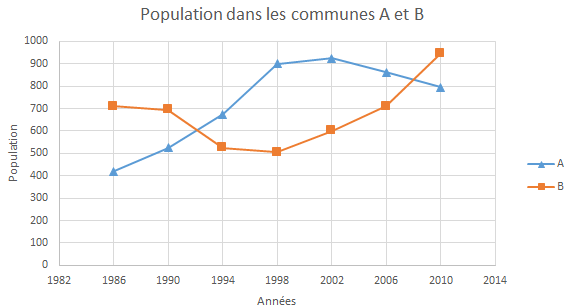
\includegraphics[scale=0.7]{./graph}
\end{center}


%\subsection{Lecture graphique}				

Répondre aux questions suivantes en utilisant uniquement le graphique ci-dessus.

\begin{questions}
	\question En quelle année, la population de la commune A a été maximale ?
	\begin{solution}
		La population de la commune A a été maximale en 2002.
	\end{solution}
	
	\question Préciser les années où les deux communes on eu le même nombre d'habitants.
	\begin{solution}
		Les deux villes ont eu la même population en 1992 et 2008.
	\end{solution}
	
	\question Quelles sont les périodes où la commune B a eu plus d'habitants que la commune A.
	\begin{solution}
		La commune B a eu plus d'habitants que la commune A entre 1986 et 1992 et entre 2008 et 2010.
	\end{solution}
	
	\question En quelle année l'écart entre le nombre d'habitants des deux communes a-t-il été le plus important.
	\begin{solution}
		L'écart entre les deux communes a été le plus important en 1998.
	\end{solution}
	
	\question Préciser, en justifiant la réponse, pendant quelle période de quatre années, la commune A a eu la plus forte augmentation de sa population.
	\begin{solution}
		La plus forte augmentation de la population de la commune A a eu lieu entre 1994 et 1998. L'angle de la pente de la courbe est la plus importante sur cette période.
	\end{solution}
\end{questions}


\section{Les sociétaires d'une mutuelle}

Une mutuelle avait \num{490000} sociétaires le 31 décembre 2006. Le nombre de sociétaires le 31 décembre à évolué les années suivantes selon le tableau ci-dessous. La deuxième colonne donne le taux d'évolution par rapport à l'année précédente, la troisième colonne, le nombre de sociétaires au 31 décembre de l'année.\\



\begin{tabular}{|c|c|c|}
	\hline
	\textbf{Année} & \textbf{\'Evolution} & \textbf{Nombre de sociétaires} \\
	\hline
	\textbf{2006} & {\LARGE $\times$} & \num{490000} \\
	\hline
	\textbf{2007} & + \num{3.24} \% & \num{506000}\\
	\hline
	\textbf{2008} & + \num{5} \% & \\
	\hline
	\textbf{2009} & &  \\
	\hline
	\textbf{2010} & + \num{2.5} \% & \num{566366} \\
	\hline
	
\end{tabular}

\begin{questions}
	\question Calculer le nombre de sociétaires le 31 décembre 2008.
	\begin{solution}
		Coefficient multiplicateur correspondant  à une hausse de \num{5} \% : $1 + \frac{5}{100}=1+\num{0.05}=\num{1.05}$.
		
		On a $\num{506000} \times \num{1.05} = \num{531300}$, donc au 31 décembre 2008, il y a \num{531300} sociétaires.
	\end{solution}
	
	\question Calculer le nombre de sociétaires le 31 décembre 2009. Arrondir à l'unité.
	\begin{solution}
		Coefficient multiplicateur : $\num{1.025}$.
		
		On a $\frac{\num{566366}}{\num{1.025}}  \approx \num{552552.1}$, soit \num{552552} sociétaires au 31 décembre 2009.
	\end{solution}
	
	\question Calculer le taux d'évolution entre le 31 décembre 2008 et le 31 décembre 2009.
	\begin{solution}
		$\frac{\num{552552} \times \num{531300}}{\num{531300}} = \num{0.04}$, soit une hausse de 4 \%.
		
		\begin{tabular}{|c|c|c|}
			\hline
			\textbf{Année} & \textbf{\'Evolution} & \textbf{Nombre de sociétaires} \\
			\hline
			\textbf{2006} & {\LARGE $\times$} & \num{490000} \\
			\hline
			\textbf{2007} & + \num{3.24} \% & \num{506000}\\
			\hline
			\textbf{2008} & + \num{5} \% & \num{531300}\\
			\hline
			\textbf{2009} & + \num{4} \% & \num{5525552} \\
			\hline
			\textbf{2010} & + \num{2.5} \% & \num{566366} \\
			\hline
			
		\end{tabular}
	\end{solution}
	
	
	\question Calculer le taux d'évolution entre le 31 décembre 2006 et le 31 décembre 2010. Arrondir à \num{0.01} \%.
	\begin{solution}
		$\frac{\num{566366}-\num{490000}}{\num{490000}}\approx \num{0.1558}$, soit une augmentation de \num{15.58} \% entre le 31 décembre 2006 et le 31 décembre 2010.
	\end{solution}
	
	
\end{questions}

\section{Population scolaire}

Dans une classe de Première, on a demandé l'âge des élèves. Les résultats obtenus ont été mis dans un tableau, mais certains ont été effacés.

\begin{center}
	\begin{tabular}{@{\ }c@{\ }|@{\ }c@{\ }|@{\ }c@{\ }|@{\ }c@{\ }|@{\ }c@{\ }|}
		\cline{2-5}
		& Pourcentage & \'Elèves & Filles & Garçons \\ \hline
		\multicolumn{1}{|c|}{16 ans} & \num{10} \% &  &   & \num{1}  \\ \hline
		\multicolumn{1}{|c|}{17 ans} &                                  &                               &                             & 12                           \\ \hline
		\multicolumn{1}{|c|}{18 ans} & \num{20} \%   &   & 3 &   \\ \hline
		\multicolumn{1}{|c|}{Total}  & \num{100} \% & \num{30}  &   & \\ \hline
	\end{tabular}	
\end{center}

\begin{questions}
	\question Combien d'élèves ont 18 ans ? Combien de garçons ont 18 ans ?
	\begin{solution}
		20 \%  des 30 élèves ont 18 ans, $30 \times \num{0.2} = 6$, donc 6 élèves ont 18 ans.
		
		$6-3=3$, il y a 3 garçons de moins de 18 ans.
	\end{solution}
	
	\question Quel est le pourcentage d'élèves ayant 17 ans ? Combien d'élèves ont 17 ans ? Combien de filles ont 17 ans ?
	\begin{solution}
		$100 - (10 + 20) = 70$, donc 70 \% des élèves ont 17 ans.
		
		$30 \times \num{0.7} = 21$, donc 21 élèves ont 17 ans.
		
		$21 - 12 = 9$, donc il y a 9 filles de 17 ans dans la classe.
	\end{solution}
	
	\question Compléter entièrement le tableau.
	\begin{solution}
		\begin{center}
			\begin{tabular}{@{\ }c@{\ }|@{\ }c@{\ }|@{\ }c@{\ }|@{\ }c@{\ }|@{\ }c@{\ }|}
				\cline{2-5}
				& Pourcentage & \'Elèves & Filles & Garçons \\ \hline
				\multicolumn{1}{|c|}{16 ans} & \num{10} \% & \num{3} & \num{2}  & \num{1}  \\ \hline
				\multicolumn{1}{|c|}{17 ans} & \num{70} \% & \num{21} & \num{9} & 12 \\ \hline
				\multicolumn{1}{|c|}{18 ans} & \num{20} \%   & 6  & 3 & 3  \\ \hline
				\multicolumn{1}{|c|}{Total}  & \num{100} \% & \num{30}  & 14  & 16\\ \hline
			\end{tabular}	
		\end{center}
	\end{solution}
\end{questions}





%\subsection{Pourcentage d'évolution}
%
%\begin{multicols}{2}
%
%\vspace*{0.1cm}	
%On s'intéresse à l'évolution de la population dans ces communes entre 2006 et 2010. Le tableau suivant indique le nombre d'habitants dans ces deux communes en 2006 et en 2010. 
%
%
%
%	\begin{tabular}{|@{\ }c@{\ }|@{\ }c@{\ }|@{\ }c@{\ }|}
%		\hline
%		\textbf{Années} & \textbf{2006} & \textbf{2010}\\
%		\hline
%		\textbf{Commune A} & \num{863} & \num{795}  \\
%		\hline 
%		\textbf{Commune B} & \num{711} & \num{947}  \\
%		\hline
%	\end{tabular}
%
%\end{multicols}	
%
%Les questions sont indépendantes.
%
%\begin{questions}
%	\question Justifier que, de 2006 à 2010, la population à baissé d'environ \num{7.9} \%.
%	\begin{solution}
%		$\dfrac{795 - 863}{863} \approx \num{-0.079} $, soit une baisse de \num{7.9} \%.
%	\end{solution}
%	
%	\question Déterminer le pourcentage d'augmentation de la population de la commune B dans cette même période (on donnera le résultat arrondi à \num{0.1} \%).
%	\begin{solution}
%		$\dfrac{947-711}{711}\approx \num{0.331}$, soit une hausse de \num{33.1}\%.
%	\end{solution}
%	
%	\question Si on considère la population des deux communes réunies, déterminer le pourcentage de cette évolution pendant durant cette période (on donnera le résultat arrondi à \num{0.1} \%).
%	\begin{solution}
%		\begin{itemize}
%			\item Population globale en 2006 : $863 + 711 = 1574$ habitants.
%			\item Population globale en 2010 : $795 + 947 = 1742$ habitants.
%			\item \'Evolution globale : $\dfrac{1742-1574}{1574} \approx \num{0.107}$, soit une hausse de \num{10.7} \%.
%		\end{itemize}
%	\end{solution}
%	
%\end{questions}





	\label{LastPage}
	

\end{document}